\input{secciones/configuracion.tex}

\usepackage{fancyhdr}
\pagestyle{fancy}
\rhead{Javier Pellejero Ortega}
\lhead{Flujo Máximo}

\begin{document}


\begin{titlepage}
\begin{center}
\vspace*{+0.75in}
\textbf{\textsc{\begin{Huge}Flujo Máximo\end{Huge}}}

\vspace*{+0.15in}
\begin{figure}[htb]
\begin{center}
\includegraphics[width=8cm]{../imagenes/complu}\\\ \\\ \\
\textsc{\textbf{\begin{LARGE}Universidad Complutense de Madrid\end{LARGE}}}\\\ \\\ \\\ \\
\textsc{\begin{Large}Métodos Algorítmicos de Resolución de Problemas\end{Large}}\\\ \\
\textsc{\begin{large}Doble Grado en Matemáticas e Ingeniería Informática\end{large}}
\end{center}
\end{figure}

\vspace*{0.35in}

\textsc{\textbf{\begin{large} Javier Pellejero \end{large}}\\}
Curso 2016-2017
\end{center}
\end{titlepage} %Portada

\blankpage
\tableofcontents\newpage %indice

\section{Introducción}
Cuando hablamos del flujo máximo de una red de flujo, estamos tratando el campo que busca la optimización de la afluencia entre vértices de un grafo, de manera que uno o varios nodos denominados sumideros reciba la mayor cantidad de dicha afluencia siempre de acuerdo a unas restricciones de capacidad entre los nodos del grafo. Es decir, limitando la capacidad de transporte de las aristas.\\

En definitiva, nos son dados unos vértices conectados o no por aristas a las que queremos asignar valores de flujo maximizando la recepción de ``mercancía'' de los vértices o nodos sumideros desde unos vértices iniciales a los que denominaremos fuentes.

\begin{defi} A continuación, definiremos una red de flujo, pues no es equivalente a un grafo cualquiera, sino que tiene unos requisitos muy concretos.
\begin{enumerate}[1)]
\item Una red de flujo es un \textbf{grafo dirigido} $G = (V,E)$ que cumple que para cada arista $(u,v)\in E$, su capacidad es mayor o igual que cero ($c(u,v) \geq 0$). Denotamos dicha propiedad como de \textbf{no negatividad}. Además, si $(u,v)\in E$ tenemos que $(v,u)\notin E$. Cabe destacar que normalizamos $c(u,v) = 0,\ \forall (u,v)\notin E$.
\item Definimos dos nodos fundamentales, el nodo \textbf{fuente} ($s$) y el nodo \textbf{sumidero} (t). Entre estos dos vértices existe al menos un camino formado por el resto de nodos de $V$; es más, para cada par de vértices de $V$ existe al menos un camino que los conecta: tenemos que el grafo $G$ es \textbf{conexo}. Por ser $G$ conexo obtenemos el resultado $\card(E)\geq \card(V)-1$, puesto que necesitamos al menos $n - 1$ aristas para unir todos los vértices de un grafo de $n$ componentes.\\  
El nodo fuente $s$ solo tiene aristas salientes, por lo que si $(u,v)\in E \implies v\neq s$, mientras que el nodo sumidero $t$ solo tiene aristas entrantes, así que si $(u,v)\in E \implies u\neq t$.
\item Definimos la \textbf{función de flujo} $\function{f}{V\times V}{\R}$ sobre el grafo $G$ que cumple:
\begin{itemize}
\item Para todo $u, v\in V$, se cumple que $0\leq f(u,v)\leq c(u,v)$. A esta propiedad la denominamos \textbf{restricción de capacidad}.
\item Si una arista $(u,v)\notin E$, entonces su función de flujo es $f(u,v)=0$.
\item Para todo $u\in V\setminus\{s,t\}$, tenemos que $\stackbin[v\in V]{}\sum f(v,u) = \stackbin[v\in V]{}\sum f(u,v)$; es decir, el flujo entrante en un nodo distinto de la fuente y el sumidero es el mismo que el flujo saliente. A esta propiedad la denominamos \textbf{conservación de flujo}.
\item Además, denotamos el valor $|f|= \stackbin[v\in V]{}\sum f(s,v)- \stackbin[v\in V]{}\sum f(v,s)$. $|f|$ es la diferencia entre el flujo saliente y el entrante de la fuente ($|\cdot|$ no denota ni cardinalidad ni valor absoluto). Aunque, en general, no tenemos aristas dirigidas hacia la fuente $\left(\stackbin[v\in V]{}\sum f(v,s)= 0\right)$, lo incluimos porque en ocasiones podemos tener redes residuales en las que el flujo dirigido a la fuente puede ser significante. Es importante destacar que $|f|= \stackbin[v\in V]{}\sum f(v,t)- \stackbin[v\in V]{}\sum f(t,v)$. Este resultado es evidente, puesto que tenemos que los vértices intermedios (distintos de $s\y t$) tienen mismo flujo saliente que entrante, por lo tanto el flujo saliente de la fuente debe ser el mismo que el entrante en el sumidero.
\end{itemize}
\end{enumerate}
\end{defi}

\begin{ejem} Veamos a continuación un ejemplo de red de flujo.\\
El grafo representado en la \textbf{Figura 1.1} se identifica con un problema de flujo máximo, donde cada arista dirigida contempla dos números. El primero de ellos se identifica con la función de flujo en $(u,v)$, es decir, $f(u,v)$; mientras que el segundo con la capacidad, $c(u,v)$.

Podemos ver que se cumplen las propiedades de \textit{restricción de capacidad} y de \textit{conservación de flujo}.
\begin{figura}\ \begin{center}\definecolor{zzttqq}{rgb}{0.15,0.35,0.15}

\begin{tikzpicture}[x=1.5cm, y=1.5cm]
	%\fill (-3.2,0) circle (0.1pt)node[anchor=east] {$20$};
	%\fill (3.2,0) circle (0.1pt)node[anchor=west] {$-20$};
    \node[circle,draw=red,fill=red!20!] (v1) at (-1.5,1.5) {$v_1$};
    \node[circle,draw=red,fill=red!20!] (v3) at (1.5,1.5) {$v_3$};
    \node[circle,draw=red,fill=red!20!] (t) at (3,0) {$t$};
    \node[circle,draw=red,fill=red!20!] (v4) at (1.5,-1.5) {$v_4$};
    \node[circle,draw=red,fill=red!20!] (v2) at (-1.5,-1.5) {$v_2$};
    \node[circle,draw=red,fill=red!20] (s) at (-3,0) {$s$};
    \draw[color=zzttqq, ultra thick, -latex]  (s) edge node[rotate = 45, above,color=black]{11/16} (v1);
	\draw[color=zzttqq, ultra thick, -latex]  (s) edge node[rotate = -45, below,color=black]{8/13} (v2);
	\draw[-latex, color=zzttqq, ultra thick]  (v2) edge node[right,color=black]{1/4} (v1);
	\draw[-latex, color=zzttqq, ultra thick]  (v1) edge node[above,color=black]{12/12} (v3);
	\draw[-latex, color=zzttqq, ultra thick]  (v2) edge node[above,color=black]{11/14} (v4);
	\draw[-latex, color=zzttqq, ultra thick]  (v3) edge node[rotate=45,above,color=black]{4/9} (v2);
	\draw[-latex, color=zzttqq, ultra thick]  (v4) edge node[right,color=black]{7/7} (v3);
	\draw[-latex, color=zzttqq, ultra thick]  (v3) edge node[rotate=-45,above,color=black]{15/20} (t);
	\draw[-latex, color=zzttqq, ultra thick]  (v4) edge node[rotate=45,below,color=black]{4/4} (t);
\end{tikzpicture}\end{center}\end{figura}

En particular, $0\leq f(u,v)\leq c(u,v)\ \forall (u,v)\in E$, y además, analizando\\
$\{v_1,v_2,v_3,v_4\}=V\setminus \{s,t\}$ tenemos:
\begin{itemize}
\item En $v_1$ tenemos la arista saliente $(v_1,v_3)$ y las entrantes $(s,v_1)\y(v_2,v_1)$ que cumplen $f(v_1,v_3)=12 = f(s,v_1)+f(v_2,v_1)$.
\item En $v_2$ tenemos las aristas salientes $(v_2,v_1)\y(v_2,v_4)$ y las entrantes $(s,v_2)\y(v_3,v_2)$ que cumplen
$f(v_2,v_1)+f(v_2,v_4)=12=f(s,v_2)+f(v_3,v_2)$.
\item En $v_3$ tenemos las aristas salientes $(v_3,t)\y(v_3,v_2)$ y las entrantes $(v_1,v_3)\y(v_4,v_3)$ que cumplen
$f(v_3,t)+f(v_3,v_2)=19=f(v_1,v_3)+f(v_4,v_3)$.
\item En $v_4$ tenemos las aristas salientes $(v_4,v_3)\y(v_4,t)$ y la entrante $(v_2,v_4)$ que cumplen
$f(v_4,v_3)+f(v_4,t)=11=f(v_2,v_4)$.
\end{itemize}
Por último señalamos que $|f| = 19$.
\end{ejem}

Para finalizar esta introducción plantearemos un problema basado en la \textbf{Figura 1.1}.\\

\begin{ejem} Los regantes murcianos, aquejados de su continua sequía, no tienen con qué regar sus preciados latifundios y campos de golf en medio del árido desierto. Para resolver este problema deciden robar ingentes cantidades de agua a la humilde población castellano-manchega. El embalse de Buendía, situado entre Cuenca y Guadalajara y de gran capacidad aunque muy mermado por los constantes saqueos murcianos, parece un lugar ideal del que abastecerse. Para hacer llegar el agua a las calurosas tierras murcianas se dispone de diversos embalses y pantanos conectados por trasvases cuyos caudales diarios en cierta unidad son conocidos. Además tenemos las siguientes conexiones:
\begin{itemize}
\item Buendía está conectado a los embalses de Entrepeñas y Beleña.
\item A su vez, Entrepeñas puede mandar agua exclusivamente al pantano de Alarcón.
\item Beleña puede enviar agua a Entrepeñas y al embalse de la Fuensanta.
\item Alarcón tiene trasvases hacia Beleña y hasta el destino final: Valdeinfierno (Murcia).
\item Por último, el embalse de la Fuensanta envía agua a Alarcón y a Valdeinfierno.
\end{itemize}
En la \textbf{Figura 1.2} están representados los embalses y pantanos, los trasvases y los caudales de los mismos. En las siguientes secciones contemplaremos algoritmos que maximizan la solución a estos problemas, es decir, nos permitirán calcular cuál es el caudal máximo diario que puede llegar a Murcia. Adelantamos que la solución máxima a este problema (que no es complicado calcular ``a ojo'') es:\\
$f(s,v_1)=12,\ f(s,v_2) = 11,\ f(v_1, v_3) = 12,\ f(v_2,v_1) = 0,\ f(v_2,v_4) = 11,\ f(v_3,v_2)=0,\\
f(v_3,t)=19,f(v_4,v_3)=7\y f(v_4,t)=4$. Por lo que podemos llevar a Murcia un máximo de 23 unidades de agua diarias.
\begin{figura}\ \begin{center}\input{figuras/figura1.2.tex}\end{center}\end{figura}
\end{ejem} % Introducción
\section{Ejemplos introductorios}
\subsection{Problema de programación lineal de dos incógnitas (en $\R^2$)}
\begin{ejem} Veamos a continuación un ejemplo de problema de programación lineal.\\

Una empresa fabrica dos tipos de productos: A y B. Los productos A y B generan unos beneficios de 100 y 600 euros respectivamente. La empresa no puede fabricar más de 4 productos diarios y además sólo recibe material suficiente para fabricar a lo sumo 2 productos A y 3 productos B al día. Veamos cuál es el beneficio máximo de la empresa a diario.\\

Planteemos el problema. Tenemos:\\
Función objetivo:
\[\mathrm{m\acute{a}x}\ z = 100x_1 + 600x_2\]
Restricciones:
\[x_1\leq 2\]
\[x_2\leq 3\]
\[x_1+x_2\leq 4\]
\[x_1,x_2\geq 0\]
No es difícil darse cuenta que cada restricción define una inecuación lineal en el plano generado por $\R^2$ que a su vez designa una parte del plano que satisface cada inecuación. Luego la región factible de este problema, si la hay, será la intersección de las partes del plano designadas por cada inecuación, como podemos observar en la \textit{figura 2.1}.
\begin{figura}\ \begin{center} \definecolor{zzttqq}{rgb}{0.6,0.2,0.}
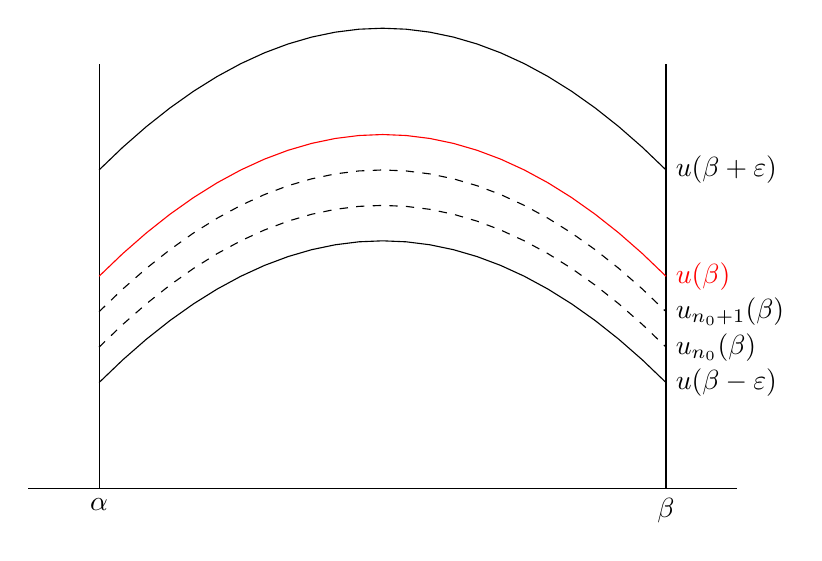
\begin{tikzpicture}[x=0.9cm,y=0.9cm]
\draw[color=black] (-1,0) -- (9,0);
\draw[color=black] (0,0) -- (0,6);
\draw[color=black] (8,0) -- (8,6);
\draw [domain=0:8, color=red] plot(\x,{-(1/8)*\x*\x+\x+3});
\draw [domain=0:8] plot(\x,{-(1/8)*\x*\x+\x+4.5});
\draw [domain=0:8] plot(\x,{-(1/8)*\x*\x+\x+1.5});
\draw [domain=0:8, dashed] plot(\x,{-(1/8)*\x*\x+\x+2.5});
\draw [domain=0:8, dashed] plot(\x,{-(1/8)*\x*\x+\x+2});
\draw[color=red] (8,3) node[anchor=west] {$u(\beta)$};
\draw (8,4.5) node[anchor=west] {$u(\beta+\varepsilon)$};
\draw (8,1.5) node[anchor=west] {$u(\beta-\varepsilon)$};
\draw (8,2) node[anchor=west] {$u_{n_0}(\beta)$};
\draw (8,2.5) node[anchor=west] {$u_{n_0+1}(\beta)$};
\draw (0,0) node[anchor=north] {$\alpha$};
\draw (8,0) node[anchor=north] {$\beta$};


\end{tikzpicture}\end{center} \end{figura}
Además, supongamos un valor $c$ fijo tal que $z(x_1,x_2)=c \iff 100x_1+600x_2=c\iff\\
\iff x_2=\dfrac{c-100x_1}{600}$, luego para cada valor $c$ que puede tomar la función $z$ tenemos otra ecuación lineal que define una recta de nivel. En dicha recta, cada par de puntos $x_1,x_2$ de la misma genera un mismo valor $c$ para nuestra función objetivo. Por lo tanto podemos trazar rectas paralelas para distintos valores de $c$ tal y como se muestra en la \textit{figura 2.2} para intuir cual es el punto donde encontramos la solución óptima (máximo) de nuestra función.
\newpage
\begin{figura}\ \begin{center}\definecolor{qqwuqq}{rgb}{0.,0.39215686274509803,0.}
\begin{tikzpicture}[x=1.0cm,y=1.0cm]
\draw[color=black] (-1,0) -- (6.5,0);
\foreach \x in {1,2,3,4,5,6}
\draw[shift={(\x,0)},color=black] (0pt,2pt) -- (0pt,-2pt) node[below] {\footnotesize $\x$};
\draw[color=black] (0,-1) -- (0,4);
\foreach \y in {1,2,3,4}
\draw[shift={(0,\y)},color=black] (2pt,0pt) -- (-2pt,0pt) node[left] {\footnotesize $\y$};
\draw[color=black] (0pt,-10pt) node[right] {\footnotesize $0$};

\draw [color=qqwuqq] (0.,3.)-- (1.,3.);
\draw [color=qqwuqq] (1.,3.)-- (2.,2.);
\draw [color=qqwuqq] (2.,2.)-- (2.,0.);
\draw [color=qqwuqq] (2.,0.)-- (0.,0.);
\draw [color=qqwuqq] (0.,0.)-- (0.,3.);

\draw [domain=-1.:5, color = blue, dashed] plot(\x,{2.5-(\x/6)}) node[anchor=south west] {$c = 1500$};
\draw [domain=-1.:5, color = blue, dashed] plot(\x,{2-(\x/6)}) node[anchor=south west] {$c = 1200$};
\draw [domain=-1.:5, color = blue, dashed] plot(\x,{1-(\x/6)}) node[anchor=south west] {$c = 600$};
\draw [domain=-1.:5, color = red, dashed] plot(\x,{3.166666667-(\x/6)}) node[anchor=south west] {$c = 1900$};

\draw [fill=black] (1,3) circle(2.5pt) node [anchor = south west] {máx $(1,3)$};

\begin{scriptsize}
\draw[color=red] (5.6, -0.5) node {$x_1$};
\draw[color=red] (-0.5,3.6) node {$x_2$};
\end{scriptsize}
\end{tikzpicture}\end{center}\end{figura}
Luego nuestra solución óptima es producir un producto A y tres productos B.
\end{ejem}

Como hemos podido observar en el ejemplo anterior, la solución óptima ha sido alcanzada en un vértice del polígono que constituye la región factible. Esto se cumplirá, en general, siempre y cuando exista una solución, lo que denominamos como problema factible, y la región factible sea acotada. Esto es extendible a $n$ variables, en $\R^3$ la solución óptima se correspondería con un vértice del poliedro que constituye la región factible y en $\R^n$ con el politopo $n$-dimensional correspondiente.\\

Y es en esto en lo que consiste el método \textit{Símplex} que comentaremos más adelante, ideado por George Dantzig en 1947. Adelantaremos brevemente explicando que este algoritmo empieza en un vértice de la región factible, en el ejemplo anterior, por ejemplo el $(0,0)$ y continua estudiando los vértices vecinos hasta encontrar uno cuyos vecinos no sean una solución mejor que él. Ese vértice se corresponde con la solución óptima. En la \textit{figura 2.3} podemos ver un esquema iterativo de como actuaría el método \textit{Símplex} en el ejemplo anterior.
\begin{figura}\ \begin{center} \begin{tikzpicture}[x=1.0cm,y=1.0cm]
\foreach \x in {1,2}
\draw[shift={(\x,0)},color=black] (0pt,2pt) -- (0pt,-2pt) node[below] {\footnotesize $\x$};
\foreach \y in {1,2,3}
\draw[shift={(0,\y)},color=black] (2pt,0pt) -- (-2pt,0pt) node[left] {\footnotesize $\y$};
\draw[color=black] (0pt,-10pt) node {\footnotesize $0$};

\draw [color=gray] (0.,3.)-- (1.,3.);
\draw [color=gray] (1.,3.)-- (2.,2.);
\draw [color=gray] (2.,2.)-- (2.,0.);
\draw [color=gray] (2.,0.)-- (0.,0.);
\draw [color=gray] (0.,0.)-- (0.,3.);


\draw [fill=black] (0,0) circle(2.5pt) node [anchor = east] {0\euro};
\draw [fill=black] (2,0) circle(2.5pt) node [anchor = west] {200\euro};
\draw [fill=black] (2,2) circle(2.5pt) node [anchor = west] {1400\euro};
\draw [fill=black] (1,3) circle(2.5pt) node [anchor = south west] {máx 1900\euro};

\draw[-triangle 45] (1.1,0)-- (1.2,0);
\draw[-triangle 45] (2,1)-- (2,1.1);
\draw[-triangle 45] (1.5,2.5)-- (1.4,2.6);
\end{tikzpicture}\end{center} \end{figura}

\subsection{Problema de programación lineal de tres incógnitas (en $\R^3$)}
\begin{ejem} Veamos un segundo ejemplo. Imaginemos que la empresa del ejemplo anterior fabrica un nuevo producto C que les genera un beneficio de 1300\euro\ por unidad vendida. Las restricciones anteriores se mantienen: el producto A se limita a 2 unidades diarias, el B a 3, de nuevo sólo podemos fabricar 4 productos diarios y además queremos añadir la restricción $x_2+3x_3\leq 6$. Luego el planteamiento del problema sería el siguiente.\\
Función objetivo:
\[\mathrm{m\acute{a}x}\ z = 100x_1 + 600x_2+1300x_3\]
Restricciones:
\[x_1\leq 2\]
\[x_2\leq 3\]
\[x_1+x_2+x_3\leq 4\]
\[x_2+3x_3\leq 6\]
\[x_1,x_2,x_3\geq 0\]

Análogamente al ejercicio anterior, donde cada restricción representaba una recta, tenemos que ahora las restricciones representan un plano y la región factible generada es, como hemos comentado antes, un poliedro, como se muestra en la \textit{figura 2.4}. Así, para $n$ variables, cada restricción representa un hiperplano en $\R^n$ que a su vez generan un politopo $n$-dimensional correspondiente a la región factible.

De igual modo, podemos asignar un valor $c$ de manera que el plano $z(x_1,x_2,x_3)=c$ se corresponde con los puntos $(x_1,x_2,x_3)$ cuyo beneficio es $c$. De nuevo, podríamos trazar distintos planos paralelos para distintos valores de $c$ para intuir cuál es la solución óptima.

Para finalizar, comentamos que para este problema tiene como solución óptima los valores $x_1=0,x_2=3,x_3=1$.
\begin{figura}\ \begin{center} 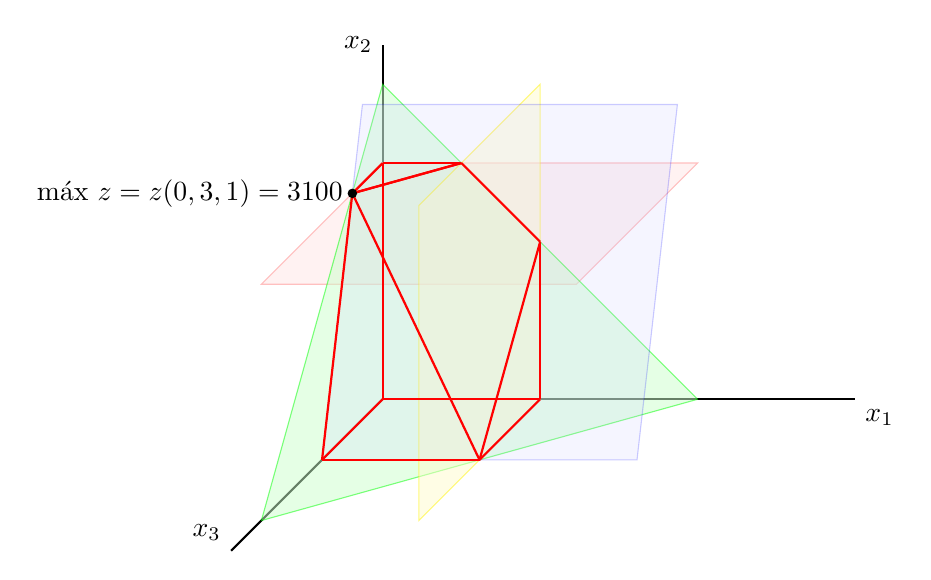
\begin{tikzpicture}
\draw[thick](0,0,0) -- (6,0,0) node[anchor=north west] {$x_1$};
\draw[thick] (0,0,0) -- (0,4.5,0) node[anchor=east] {$x_2$};
\draw[thick] (0,0,0) -- (0,0,5) node[anchor=south east] {$x_3$};

\filldraw[draw=pink,fill=pink!20] (0,3,0) -- (4,3,0) -- (4,3,4) -- (0,3,4) -- (0,3,0);
\filldraw[draw=green,fill=green!20, opacity=0.5] (4,0,0) -- (0,0,4) -- (0,4,0) -- (4,0,0);
\filldraw[draw=yellow,fill=yellow!20, opacity=0.5] (2,0,0) -- (2,0,4) -- (2,4,4) -- (2,4,0) -- (2,0,0);
\filldraw[draw=blue,fill=blue!20, opacity=0.2] (0,0,2) -- (4,0,2) -- (4,4,0.667) -- (0,4,0.667) --(0,0,2);

\draw[thick, red] (0,0,0) -- (2,0,0);
\draw[thick, red] (0,0,0) -- (0,3,0);
\draw[thick, red] (0,3,0) -- (1,3,0);
\draw[thick, red] (1,3,0) -- (2,2,0);
\draw[thick, red] (2,2,0) -- (2,0,0);
\draw[thick, red] (0,0,0) -- (0,0,2);
\draw[thick, red] (0,0,2) -- (2,0,2);
\draw[thick, red] (2,0,2) -- (2,0,0);
\draw[thick, red] (0,0,2) -- (0,3,1);
\draw[thick, red] (0,3,1) -- (0,3,0);
\draw[thick, red] (0,3,1) -- (2,0,2);
\draw[thick, red] (2,0,2) -- (2,2,0);
\draw[thick, red] (0,3,1) -- (1,3,0);

\draw[thick, red] (0,3,1) -- (1,3,0);

\draw [fill=black] (0,3,1) circle(1.5pt) node[anchor=east]{máx $z=z(0,3,1)=3100$\euro};

            

\end{tikzpicture}\end{center} \end{figura}
\end{ejem} % Modelación de problemas
\section{Representación de una red de flujo como problema de programación lineal}

Aprovechando el tema de \textit{programación lineal} que traté el cuatrimestre anterior para la composición de mi trabajo, me gustaría, antes de comenzar con los algoritmos de resolución de problemas de flujo, plantear un ejemplo en el que convertimos una de estas redes en un problema de programación lineal.\\

En el anterior trabajo comenté un problema de mínimo coste en una red de flujo, similar al problema que estamos tratando. Con un grafo con características similares al introducido en la primera sección, podemos plantear un problema de mínimo coste en el que tenemos prefijadas una oferta del nodo fuente y una demanda del nodo sumidero cuyos valores son idénticos.

En este caso no tratamos de calcular el máximo flujo que podemos llevar hasta el nodo sumidero, si no que el objetivo es minimizar los costes de transportar la prefijada mercancía a través de las aristas disponibles que tienen una capacidad y unos costes por unidad de mercancía transportada conocidos.\\

No indagaremos más sobre este tipo de problemas puesto que ya fueron expuestos en el trabajo anterior, pero las ecuaciones lineales resultantes son similares en ambos problemas. Sin más dilación plantearemos una red de flujo máximo como un programa lineal.\\

Sea un grafo $G=(V,E)$ con capacidades $c(u,v)$ conocidas $\forall u,v\in V, u\neq v$ y denotamos $f(u,v)$ el suministro de mercancía que mandamos del vértice $u$ al $v$.\\
Recordemos que un programa lineal busca maximizar o minimizar una función objetivo (en nuestro caso maximizar) de acuerdo a unas restricciones. Obtengamos primero nuestra función objetivo:\\

Nuestro cumplido es hacer llegar al vértice sumidero el mayor número de unidades de mercancía posible, es decir, debemos maximizar el flujo entrante en el sumidero, o debido a su equivalencia (vista en la \textit{Sección 1}), maximizar el flujo saliente de la fuente. Esto es:
\[\max z = |f| = \stackbin[v\in V]{}\sum f(s,v)- \stackbin[v\in V]{}\sum f(v,s)\]

Veamos ahora las restricciones. En primer lugar tenemos que $\forall u,v\in V$:
\[0\leq f(u,v)\leq c(u,v)\]

Y en segundo lugar, para cada vértice $u\in V$, tenemos:
\[\stackbin[v\in V]{}\sum f(u,v)- \stackbin[v\in V]{}\sum f(v,u)=0\]

\begin{ejem} Veamos para acabar un ejemplo concreto, representemos el problema de los embalses de la \textit{Sección 1} como un problema de programación lineal.\\

Nuestra función objetivo busca sacar el máximo posible de agua de Buendía, así, tenemos:
\[\max z = f(s,v_1)+f(s,v_2)\equiv \max z'=f(v_3,t)+f(v_4,t)\]

En cuanto a restricciones tenemos:
\begin{align*}
0\leq f(s,v_1)\leq& c(s,v_1)		&  0\leq f(v_2,v_1)\leq& c(v_2,v_1)         &  0\leq f(v_3,t)\leq& c(v_3,t)\\
0\leq f(s,v_2)\leq& c(s,v_2)        &  0\leq f(v_2,v_4)\leq& c(v_2,v_4)			&  0\leq f(v_4,v_3)\leq& c(v_4,v_3)\\	
0\leq f(v_1,v_3)\leq& c(v_1,v_3)  	&  0\leq f(v_3,v_2)\leq& c(v_3,v_2)			&  0\leq f(v_4,t)\leq& c(v_4,t)
\end{align*}
\begin{align*}
f(s,v_1)+f(s,v_2)=&f(v_3,t)+f(v_4,t)& f(v_1,v_3)=&f(s,v_1) + f(v_2,v_1)\\
f(v_2,v_1)+f(v_2,v_4)=&f(s,v_2)+f(v_3,v_2)&f(v_3,v_2)+f(v_3,t)=&f(v_1,v_3)+f(v_4,v_3)
\end{align*}
\[f(v_4,v_3)+f(v_4,t)=f(v_2,v_4)\]

Una vez formulado el problema ya estaríamos listos para normalizar el problema a forma estándar y aplicar el algoritmo \textit{Símplex} o cualquier otro método de resolución de problemas de programación lineal. Como hemos indicado anteriormente, todo esto ya fue tratado en las notas presentadas para el cuatrimestre anterior y no entraremos en más detalle.
\end{ejem} % Representación de una red de flujo como problema de programación lineal
\section{El método Ford-Fulkerson}
Vamos a introducir en esta sección el método de \textit{\textbf{Ford-Fulkerson}} para la resolución de problemas de flujo máximo sobre un grafo $G=(V,E)$. Se trata de un método iterativo que comienza con una función de flujo nula ($f(u,v)= 0\ \forall u,v\in V$) y en cada iteración incrementa el valor del flujo en $G$ mediante la búsqueda de caminos o cadenas de aumento en un grafo asociado $G_f$ que denotamos como \textbf{red residual}, que definiremos a continuación.\\

La idea del método es facilitar la búsqueda de aristas de $G$ a las que podamos modificar su valor para aumentar el flujo de $G$, en definitiva, aumentar $|f|$. El cambio de flujo en dichas aristas en cada iteración no es necesariamente un incremento, sino que en multitud de ocasiones decreceremos el flujo de una o más determinadas aristas para mejorar $|f|$. El método finaliza una vez no encontremos más cadenas de aumento.\\

\subsection{Red residual y función de aumento de flujo}

\begin{defi} Definamos a continuación el concepto de \textbf{red residual}.

Dado un grafo $G=(V,E)$ y un flujo $f$, definimos la red residual $G_f=(V,E_f)$ como el grafo de aristas de $G$ con capacidades que representan el cambio de flujo que podemos realizar sobre las aristas de $G$. Una arista del grafo $G$ puede admitir un aumento adicional de flujo igual a la capacidad de la arista menos el flujo que ya transporta. Así, las únicas aristas que pertenecen a $E_f$ son las que admiten más flujo. Definimos entonces\\
$c_f(u,v)=c(u,v)-f(u,v)\ \forall u,v\in V$.\\

Sin embargo, como comentamos anteriormente, existe la posibilidad de que queramos decrecer el flujo de una arista para obtener el bien mayor de maximizar el flujo de nuestra red. Surge así la necesidad de añadir ciertas aristas a $G_f$ que no pertenecen a $G$. Para representar el posible decrecimiento de una arista $(u,v)\in E$ con flujo positivo tomaremos $(v,u)\in E_f$ de manera que $c_f(v,u)=f(u,v)$. Es decir, podemos llevar flujo de $v$ a $u$, en sentido contrario al original, que sería equivalente a hacer disminuir el flujo de $(u,v)$. Definamos formalmente la capacidad de cada arista de $G_f$:
\[c_f(u,v)=\tripleleft{c(u,v)-f(u,v)& \mathrm{si\ }(u,v)\in E}{f(v,u) &\mathrm{si\ }(v,u)\in E}{0&\mathrm{en\ otro\ caso}}\]
Recordemos que si $(u,v)\in E\implies (v,u)\notin E$, luego la anterior definición está bien construida.

\begin{ejem} Sea una arista $(u,v)$ de cierto grafo $G$ tal que su capacidad $c(u,v) =16$ y su flujo $f(u,v)=11$, entonces $c_f(u,v) = 5\y c_f(v,u)=11$.
\end{ejem}

Por último, recalcar que una vez calculado $c_f(u,v)\ \forall u,v\in V$ podemos definir\\
$E_f=\{(u,v)\in V\times V\ |\ c_f(u,v)>0\}$ y que por la definición, es fácil ver que\\
$\card(E_f)\leq 2\cdot\card(E)$.
\end{defi}

Definida la red residual por el grafo $G_f$, tenemos que $G_f$ no cumple la definición de red de flujo dada en la \textit{Sección 1}, puesto que en múltiples ocasiones nos encontraremos con $(u,v),(v,u)\in E_f$ para ciertos $u,v\in V$. Sin embargo, podemos definir una función de flujo $f'$ sobre ella de manera que cumpla la propiedad de \textbf{restricción de capacidad} que es la que nos interesa de cara al desarrollo de estas ideas.

\begin{defi} Definimos el \textbf{aumento de flujo de $f$ por $f'$}, que denotamos $(f\uparrow f')$ como:
\[(f\uparrow f')(u,v)=\doubleleft{f(u,v)+f'(u,v)-f'(v,u)& \mathrm{si\ }(u,v)\in E}{0&\mathrm{en\ otro\ caso}}\]
\end{defi}

\begin{proposicion} Sea $G=(V,E)$ un grafo de una red de flujo y $f$ su función de flujo. Sea $G_f$ la red residual de $G$ inducida por $f$ y $f'$ la función de flujo de $G_f$. Entonces la función de aumento $f\uparrow f'$ es una función de flujo sobre $G$ bien definida con valor $|f\uparrow f'|=|f|+|f'|$.\\

La demostración de esta proposición, pese a no ser tediosa, no es lo suficientemente corta como para incluirse en estas notas. Puede consultarse en \textit{Cormen, T., Leiserson, C., Rivest, R. and Stein, C. (2009). Introduction to algorithms}, capítulo 26, páginas 717, 718 y 719.
\end{proposicion}

\subsection{Cadenas de aumento y cortes}

\begin{defi} Procedamos a definir el concepto de \textbf{cadenas de aumento}.\\
Una cadena de aumento $p$ es un camino entre los vértices $s$ y $t$ de la red residual $G_f$. Por cómo hemos definido $G_f\y f'$, una cadena de aumento $p$ de $G_f$ es un incremento de flujo para la red de $G$ siempre que no violemos ninguna capacidad $c_f(u,v)$.\\

Para asegurarnos de que dicha violación de capacidad no ocurra, definimos la \textbf{capacidad residual de $p$} como $c_f(p)=\min\{c_f(u,v)\ |\ (u,v)\mathrm{\ est\acute{a}\ en\ } p\}$.
\end{defi}

Veamos en la siguiente proposición un argumento más preciso de qué hemos logrado al encontrar una cadena de aumento.

\begin{proposicion} Sea $G=(V,E)$ una red de flujo y $f$ un flujo en $G$. Sea $G_f$ la red residual de $G$ y $p$ una cadena de aumento en $G_f$. Definamos $\function{f_p}{V\times V}{\R}$ tal que \[f_p(u,v)=\doubleleft{c_f(p)& \mathrm{si\ }(u,v)\mathrm{\ est\acute{a}\ en\ } p}{0&\mathrm{en\ otro\ caso}}\]

Entonces $f_p$ es una función de flujo en $G_f$ con valor $|f_p|=c_f(p)>0$ y $f\uparrow f_p$ es un aumento de flujo de $f$. Además tenemos que $|f\uparrow f_p|=|f|+|f_p|>|f|$, por lo que hemos mejorado el flujo en $G$ que teníamos anteriormente.
\end{proposicion}

\begin{defi} Concluyamos las definiciones de esta sección explicando en qué consiste un corte.\\
Un \textbf{corte $(S,T)$ de una red de flujo} $G=(V,E)$ es una partición de $V$ en dos conjuntos $S \y T=V\setminus S$ (es decir, se cumple que $S\cup T=V \y S\cap T=\emptyset$) tal que $s\in S\y t\in T$.

Si $f$ es un flujo en $G$, definimos el \textbf{flujo neto} $f(S,T)$ a través del corte $(S,T)$ como
\[f(S,T)=\stackbin[u\in S]{}\sum\stackbin[v\in T]{}\sum f(u,v)-\stackbin[u\in S]{}\sum\stackbin[v\in T]{}\sum f(v,u)\]

Además definimos la \textbf{capacidad} del corte $(S,T)$ como $c(S,T)=\stackbin[u\in S]{}\sum\stackbin[v\in T]{}\sum c(u,v)$.
\end{defi}

\begin{proposicion} Sea $f$ un flujo en una red $G$ y $(S,T)$ un corte cualquiera de $G$, entonces el flujo neto $f(S,T)=|f|$.

De nuevo la demostración puede verse en \textit{Cormen, T., Leiserson, C., Rivest, R. and Stein, C. (2009). Introduction to algorithms}, capítulo 26, página 722.\\

Es decir, nos es indiferente el corte que realicemos en $G$, siempre obtendremos el mismo flujo neto que es equivalente al flujo $|f|$ de $G$. Además no es difícil comprobar que\\ $|f|=f(S,T)\leq c(S,T)$.
\end{proposicion}

A continuación enunciaremos un importante teorema que nos ayudará a saber si ya tenemos o no un flujo máximo para nuestra red $G$, pero antes veremos algunos ejemplos gráficos sobre el material introducido en esta sección.
\newpage
\begin{figura}\ \begin{center}\input{figuras/figura4.1.tex}\end{center}\end{figura}

En la \textbf{Figura 4.1} hemos representado una red de flujo $G=(V,E)$ con una función de flujo y sus capacidades. Veamos como queda su red residual $G_f$.

\begin{figura}\ \begin{center}\definecolor{zzttqq}{rgb}{0.15,0.35,0.15}

\begin{tikzpicture}[x=1.5cm, y=1.5cm]
	%\fill (-3.2,0) circle (0.1pt)node[anchor=east] {$20$};
	%\fill (3.2,0) circle (0.1pt)node[anchor=west] {$-20$};
    \node[circle,draw=red,fill=red!20!] (v1) at (-1.5,1.5) {$v_1$};
    \node[circle,draw=red,fill=red!20!] (v3) at (1.5,1.5) {$v_3$};
    \node[circle,draw=red,fill=red!20!] (t) at (3,0) {$t$};
    \node[circle,draw=red,fill=red!20!] (v4) at (1.5,-1.5) {$v_4$};
    \node[circle,draw=red,fill=red!20!] (v2) at (-1.5,-1.5) {$v_2$};
    \node[circle,draw=red,fill=red!20] (s) at (-3,0) {$s$};
    \DoubleLine{s}{v1}{latex-, color=zzttqq, ultra thick}{7}{-latex, color=zzttqq, ultra thick}{9}
    \DoubleLine{s}{v2}{latex-, color=zzttqq, ultra thick}{11}{-latex, color=zzttqq, ultra thick}{2}
    \DoubleLine{v2}{v1}{latex-, color=zzttqq, ultra thick}{1}{-latex, color=zzttqq, ultra thick}{3}
    \DoubleLine{v1}{v3}{latex-, color=zzttqq, ultra thick}{8}{-latex, color=zzttqq, ultra thick}{4}
    \DoubleLine{v2}{v4}{latex-, color=zzttqq, ultra thick}{10}{-latex, color=zzttqq, ultra thick}{4}
	%\draw[-latex, color=zzttqq, ultra thick]  (v2) edge node[above,color=black]{10/14} (v4);
	\draw[-latex, color=zzttqq, ultra thick]  (v3) edge node[rotate=45,above,color=black]{9} (v2);
	\draw[-latex, color=zzttqq, ultra thick]  (v3) edge node[right,color=black]{7} (v4);
    \DoubleLine{v3}{t}{latex-, color=zzttqq, ultra thick}{15}{-latex, color=zzttqq, ultra thick}{5}
	\DoubleLine{v4}{t}{latex-, color=zzttqq, ultra thick}{3}{-latex, color=zzttqq, ultra thick}{1}
\end{tikzpicture}\end{center}\end{figura}

En la \textbf{Figura 4.2} tenemos representado el grafo residual $G_f$ derivado del grafo $G$ y su función de flujo $f$.
\newpage
\begin{figura}\ \begin{center}\definecolor{zzttqq}{rgb}{0.15,0.35,0.15}

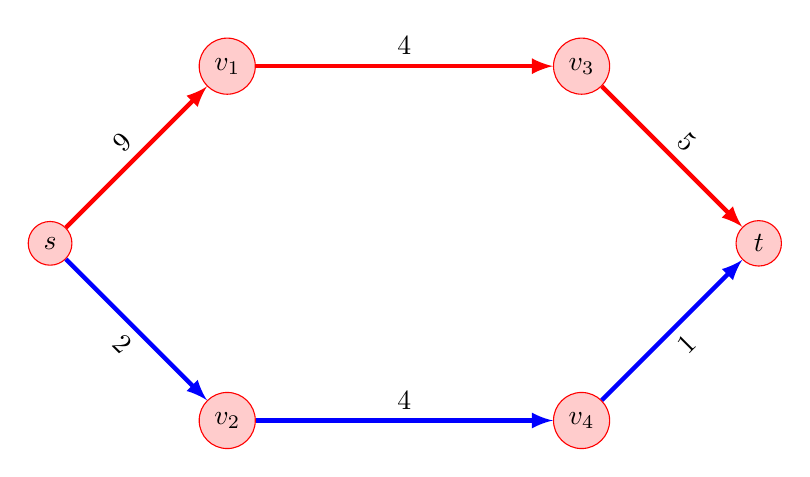
\begin{tikzpicture}[x=1.5cm, y=1.5cm]
	%\fill (-3.2,0) circle (0.1pt)node[anchor=east] {$20$};
	%\fill (3.2,0) circle (0.1pt)node[anchor=west] {$-20$};
    \node[circle,draw=red,fill=red!20!] (v1) at (-1.5,1.5) {$v_1$};
    \node[circle,draw=red,fill=red!20!] (v3) at (1.5,1.5) {$v_3$};
    \node[circle,draw=red,fill=red!20!] (t) at (3,0) {$t$};
    \node[circle,draw=red,fill=red!20!] (v4) at (1.5,-1.5) {$v_4$};
    \node[circle,draw=red,fill=red!20!] (v2) at (-1.5,-1.5) {$v_2$};
    \node[circle,draw=red,fill=red!20] (s) at (-3,0) {$s$};
    \draw[color=red, ultra thick, -latex]  (s) edge node[rotate = 45, above,color=black]{9} (v1);
	\draw[color=blue, ultra thick, -latex]  (s) edge node[rotate = -45, below,color=black]{2} (v2);
	\draw[-latex, color=red, ultra thick]  (v1) edge node[above,color=black]{4} (v3);
	\draw[-latex, color=blue, ultra thick]  (v2) edge node[above,color=black]{4} (v4);
	\draw[-latex, color=red, ultra thick]  (v3) edge node[rotate=-45,above,color=black]{5} (t);
	\draw[-latex, color=blue, ultra thick]  (v4) edge node[rotate=45,below,color=black]{1} (t);
\end{tikzpicture}\end{center}\end{figura}

En la \textbf{Figura 4.3} hemos dibujado dos cadenas de aumento (en rojo y azul respectivamente). Si denotamos el camino rojo como $p_1$, tenemos que $c_f(p_1)=4$ y que $f_{p_1}(s,v_1)=f_{p_1}(v_1,v_3)=f_{p_1}(v_3,t)=4$. Mientras que si denotamos el azul por $p_2$, obtenemos $c_f(p_2)=1$ y que $f_{p_2}(s,v_2)=f_{p_1}(v_2,v_4)=f_{p_1}(v_4,t)=1$. Nos quedaremos por ejemplo con el rojo y así surge el flujo de aumento $f\uparrow f_{p_2}$ presente en la \textbf{Figura 4.4}.

\begin{figura}\ \begin{center}\input{figuras/figura4.4.tex}\end{center}\end{figura}

En este caso hemos aumentado de un flujo $|f|=18$ a $22$. Podríamos redibujar la nueva red residual del grafo $G$ resultante y continuar buscando otra cadena de aumento, así hasta que no encontráramos ninguna otra.
\newpage
\begin{figura}\ \begin{center}\definecolor{zzttqq}{rgb}{0.15,0.35,0.15}

\begin{tikzpicture}[x=1.5cm, y=1.5cm]
	\fill (0.15,-2.4) circle (0.1pt)node[anchor=west] {$T\rightarrow$};
	\fill (-0.15,-2.4) circle (0.1pt)node[anchor=east] {$\leftarrow S$};
	\node[circle,draw=red,fill=red!20] (s) at (-3,0) {$s$};
    \node[circle,draw=red,fill=red!20!] (v1) at (-1.5,1.5) {$v_1$};
    \node[circle,draw=red,fill=red!20!] (v2) at (-1.5,-1.5) {$v_2$};
    
    \node[circle,draw=blue,fill=blue!20!] (v3) at (1.5,1.5) {$v_3$};
    \node[circle,draw=blue,fill=blue!20!] (v4) at (1.5,-1.5) {$v_4$};
    \node[circle,draw=blue,fill=blue!20!] (t) at (3,0) {$t$};
    
    \draw[color=zzttqq, ultra thick, -latex]  (s) edge node[rotate = 45, above,color=black]{11/16} (v1);
	\draw[color=zzttqq, ultra thick, -latex]  (s) edge node[rotate = -45, below,color=black]{11/13} (v2);
	\draw[-latex, color=zzttqq, ultra thick]  (v2) edge node[right,color=black]{1/4} (v1);
	\draw[-latex, color=zzttqq, ultra thick]  (v1) edge node[above,color=black]{12/12} (v3);
	\draw[-latex, color=zzttqq, ultra thick]  (v2) edge node[above,color=black]{10/14} (v4);
	\draw[-latex, color=zzttqq, ultra thick]  (v3) edge node[rotate=45,above,color=black]{0/9} (v2);
	\draw[-latex, color=zzttqq, ultra thick]  (v4) edge node[right,color=black]{7/7} (v3);
	\draw[-latex, color=zzttqq, ultra thick]  (v3) edge node[rotate=-45,above,color=black]{19/20} (t);
	\draw[-latex, color=zzttqq, ultra thick]  (v4) edge node[rotate=45,below,color=black]{3/4} (t);
	\draw[color=gray, ultra thick, dashed]  (0, 2.5) edge (0,-2.5);
\end{tikzpicture}\end{center}\end{figura}

Para finalizar con estos ejemplos, en la \textbf{Figura 4.5} hemos practicado un corte $(S,T)$ sobre el grafo de la \textbf{Figura 4.4}. Su flujo neto $f(S,T)=\stackbin[u\in S]{}\sum\stackbin[v\in T]{}\sum f(u,v)-\stackbin[u\in S]{}\sum\stackbin[v\in T]{}\sum f(v,u)=\\= f(v_1,v_3)+f(v_2,v_4)-f(v_3,v_2)=12+10-0=22$. Mientras que su capacidad de corte es $c(S,T)=\stackbin[u\in S]{}\sum\stackbin[v\in T]{}\sum c(u,v)=c(v_1,v_3)+c(v_2,v_4)=12+14=26$.

\subsection{Teorema del flujo máximo y corte mínimo}
\begin{teor} Sea $f$ un flujo en una red $G=(V,E)$ con una fuente $s$ y un sumidero $t$, entonces son equivalentes:
\begin{enumerate}[1)]
\item $f$ es máximo flujo en $G$.
\item La red residual $G_f$ no contiene cadenas de aumento.
\item $|f|=c(S,T)$ para cierto corte $(S,T)$ de $G$.
\end{enumerate}
\begin{proof}\ 
\begin{itemize}
\item (1 $\implies$ 2) Supongamos que no. Supongamos que $f$ es flujo máximo en $G$ y existe una cadena de aumento $p$ en $G_f$. Entonces existe una función de flujo $f_p$ en $G_f$ y por la \textbf{Proposición 4.2}, la función de flujo $f\uparrow f_p$ está bien definida sobre $G$ y $|f\uparrow f_p|=|f|+|f_p|>|f|$ lo que contradice que $f$ sea flujo máximo.
\newpage
\item (2 $\implies$ 3) Supongamos que no existen cadenas de aumento, esto es que no hay ningún camino de $s$ a $t$ en $G_f$. Definimos $S=\{v\in V\ |\ $existe un camino de $s$ a $v\}$, evidentemente $t\notin S$ puesto que no existe ningún camino de $s$ a $t$ y definimos $T=V\setminus S$. $(S,T)$ es un corte y para cada par $(u,v)$ con $u\in S, v\in T$, $(u,v)\notin E_f$, puesto que no existe un camino entre ellos. Tenemos que si $(u,v)\in E$, por lo anterior, $f(u,v)=c(u,v)$. Si $(v,u)\in E$, entonces $f(v,u)=0$ ya que en otro caso $(u,v)$ pertenecería a $E_f$ y esto no es posible. Así tenemos que\\ $f(S,T)=\stackbin[u\in S]{}\sum\stackbin[v\in T]{}\sum f(u,v)-\stackbin[u\in S]{}\sum\stackbin[v\in T]{}\sum f(v,u)=\stackbin[u\in S]{}\sum\stackbin[v\in T]{}\sum f(u,v)=\stackbin[u\in S]{}\sum\stackbin[v\in T]{}\sum c(u,v)=c(S,T)$.
\item (3 $\implies$ 1) Por la \textbf{Proposición 4.3} tenemos que $|f|\leq c(S,T)$ para cualquier corte $(S,T)$ de $G$, como $|f|= c(S,T)\implies f$ es máximo.
\end{itemize}
\end{proof}
\end{teor}

\subsection{Implementación en pseudocódigo del método Ford-Fulkerson y complejidad}

Para finalizar esta sección veamos un algoritmo del método \textbf{\textit{Ford-Fulkerson}} implementado en pseudocódigo. Como observaremos, el código es bastante simple.

\begin{algorithmic}[1]
\State /*********************
\State	* FordFulkerson ($G,s,t,f$)
\State *********************/
\For {cada arista $(u,v) \in G.E$}
	\State $f(u,v) = 0$
\EndFor
\While {$\exists p$ cadena de aumento en $G_f$}
	\State $c_f(p)=\min\{c_f(u,v)\ |\ (u,v)$ está en $p\}$
	\For {cada arista $(u,v)$ en $p$}
		\If {$(u,v)\in G.E$}
			\State $f(u,v) = f(u,v) +c_f(p)$
		\Else
			\State $f(u,v) = f(u,v) -c_f(p)$
		\EndIf
	\EndFor
\EndWhile
\end{algorithmic}
\ 

Para la búsqueda del camino podemos utilizar uno de los algoritmos de búsqueda en profundidad sobre el grafo $G_f$ vistos en clase. Recordemos que el coste de cualquiera de estas búsquedas tiene $\mathcal{O}(V+E')$ que podemos reducir a $\mathcal{O}(E')$, puesto que en general tendremos muchas más aristas que vértices. Además recordemos que $\card(E')\leq2\cdot\card(E)$, luego $\mathcal{O}(E')=\mathcal{O}(2E)=\mathcal{O}(E)$.
Por último, el número máximo de veces que buscaremos si hay o no este camino será cuando lleguemos a alcanzar el flujo máximo, es decir, $|f|$. Luego el orden de \textbf{\textit{Ford-Fulkerson}} puede ser definido como $\mathcal{O}(|f|E)$. % El método Ford-Fulkerson
\section{Bibliografía}

\begin{enumerate}
\item Cormen, T., Leiserson, C., Rivest, R. and Stein, C. (2009). Introduction to algorithms. 3rd ed. Cambridge, Massachusetts: The MIT Press.
\item Dasgupta, S., Papadimitriou, C. and Vazirani, U. (2011). Algorithms. 1st ed. Boston: McGraw-Hill Higher Education.
\item Notas de la asignatura \textit{investigación operativa} impartida por \textit{doña María Inés Sobrón Fernández} en la \textit{Facultad de Matemáticas} de la \textit{Universidad Complutense de Madrid} durante el curso 2016-2017.
\end{enumerate} % Algoritmo de Edmonds-Karp
\section{Algoritmos push–relabel y  relabel-to-front}
En esta última sección vamos a ver, sin profundizar, unos algoritmos con mejores costes que los vistos anteriormente.
El algoritmo \textit{push–relabel} trabaja en $\mathcal{O}(V^2E)$ mejorando el $\mathcal{O}(VE^2)$ del algoritmo \textit{Edmonds-Karp} (recordemos que en general el cardinal de $V$ es mucho menor que el cardinal de $E$). Veremos también el algoritmo \textit{relabel-to-front}, variación de \textit{push–relabel} con mejor coste: $\mathcal{O}(V^3)$.
\subsection{Algoritmo push–relabel}
En este algoritmo no son válidas algunas de las definiciones dadas en la \textit{Sección 1}. Para empezar, sustituimos la función de flujo por la siguiente.

\begin{defi} Definimos la función \textbf{preflujo} como $\function{f}{V\times V}{\R}$ que cumple:
\begin{itemize}
\item $\forall u\in V\setminus\{s\}$ tenemos que $\stackbin[v\in V]{}\sum f(v,u)-\stackbin[v\in V]{}\sum f(u,v) \geq 0$.
\end{itemize}

Definimos como \textbf{exceso de flujo} al valor $e(u)=\stackbin[v\in V]{}\sum f(v,u)-\stackbin[v\in V]{}\sum f(u,v)$. Decimos que un vértice $u\in V\setminus\{s,t\}$ está \textbf{desbordado} si $e(u)>0$.
\end{defi}

\begin{defi} Sea un preflujo $f$ sobre una red de flujo $G(V,E)$, definimos \textbf{función de peso} o \textbf{función de distancia} como $\function{h}{V}{\N}$ que cumple:
\begin{itemize}
\item $h(s) = \card(V)$.
\item $h(t) = 0$.
\item $h(u)\leq h(v) + 1$ para toda arista residual $(u,v)\in E_f$. Luego si $h(u) > h(v) +1\implies\\\implies (u,v)\notin E_f$.
\end{itemize}
\end{defi}

No entraremos más en detalle acerca de este algoritmo, procederemos a explicar la intuición del mismo.

El algoritmo trata el problema vértice a vértice trabajando con sus vecinos en lugar de con todo el grafo. El objetivo es llevar la mayor cantidad posible de flujo de un vértice a sus vecinos, de ahí que pueda producirse el desbordamiento de flujo en cada iteración. Siempre llevamos flujo de vértices con ``pesos'' más altos a ``pesos'' más bajos (``cuesta abajo''), es decir, según el valor de $h$ en dos determinados vértices llevamos flujo de uno a otro o no. A esta operación se le denomina \textbf{empuje} (\textit{push}). Cuando no tenemos vértices con pesos más bajos a los que llevar flujo entra en juego la operación de \textbf{reetiquetado} (\textit{relabel}), consistente en aumentar el peso del vértice en el que nos encontramos, y comenzamos de nuevo nuestra operación de empuje.

\subsection{Algoritmo relabel-to-front}

Este algoritmo es una variante de \textit{push–relabel}. En este caso, en lugar de un recorrido vértice a vértice, poseemos una lista enlazada con los vértices de la red ordenados por su admisión de flujo. El método recorre la lista y realiza la operación de empuje sobre los nodos con desbordamiento. Si un nodo es reetiquetado, se mueve al principio de la lista y comenzamos a recorrer de nuevo la lista desde el principio. % Algoritmos push–relabel y  relabel-to-front
\section{Bibliografía}

\begin{enumerate}
\item \textit{Cormen, T., Leiserson, C., Rivest, R. and Stein, C. (2009). Introduction to algorithms, chapter 26}.
\item  \textit{Sedgewick, R., Wayne, K. (2011). Algorithms, chapter 6.4}.
\end{enumerate} % Bibliografía

\end{document}